\documentclass{article}
\usepackage{graphicx}

\begin{document}
\title{Trading Game Group Project: Project Report}
\author{Jack Bracewell, Craig Ellis, Milan Misak}
\date{}

\maketitle
\vspace{1.5cm}
\tableofcontents
\clearpage

\section{Introduction}
We set out from the beginning to make a game, and to make it original. In addition to being original, we wanted the game to be fun to play, and of course be online multiplayer. We also wanted the game to be lightweight in terms of connection demands, and in terms of demand placed on any server we might use. Our final objective was that the game must be visually pleasing, which would inevitably mean taking more time and care in the artwork than programmers usually do. \\ \\
To meet our low networking demands, we decided to make a turn based game. This would make the latency requirements very low and would allow anyone in the world to play against each other, regardless of location. For example, if someone is playing a latency critical game such as Call of Duty, and the client and host are in England and Brazil respectively, then the latency will cause the game to be unplayable or at least have a severely degraded experience. This is something we wanted to be sure of avoiding. \\ \\
Eventually we settled on making a game based on defending a certain location, and decided to force player co-operation in preventing a house from being invaded by enemies. 


\section{Project Management}

\subsection{Group Structure}
Initially, we split into a pair and a single person, with Craig and Jack working on the graphics, artwork and client-side representation of the game. Milan focused on creating the layout for the website, and lay a structure for the back end Django application. As the project progressed, everybody began to help with anything that needed doing, as many areas of work overlapped.

\subsection{Git}
We used git as the version control for our project; more specifically the online git hosting service, github. Git is simple and easy to use, and we have become very familiar with it from previous group projects. It is a distributed version control system which makes it great for working independently of other team members.

\subsection{PivotalTracker}
To organise our team, we used a project management software called Pivotal Tracker. This allowed us to create tasks, set a priority and a difficulty for each task, and to assign group members to complete each task. Pivotal Tracker automatically arranges tasks to maximise efficient time use, based on previous performance. A list of current tasks is maintained, along with a backlog. Tasks are made 'current' when it is predicted that there is enough free space (For example, if the group works quickly, there will be a larger capacity in 'current tasks'. If the group works slowly, Pivotal Tracker makes sure there are fewer current tasks to complete).

\subsection{Other tools}
TODO: this?

\subsection{Implementation Languages}
We chose to write the front end in Javascript and HTML5, and we chose to also use this as a basis for the graphics instead of using Flash or a Java applet. This is because unlike the previous 2 choices, a HTML5-based game will load faster and, as a new technology standard, it is gaining good web browser support. People are already talking about stopping flash support - on mobile devices in particular. \\ \\
We chose to use Django for the back end because some of us have had previous experience using the platform, and because of its many useful features. For example, Object-relational mapping (ORM) allows us to effectively deal with database queries while also having a good object-oriented design for the application's entities. With view templates we can easily create HTML parts of the website and with URL mapping we have full control over the URLs used by the website (so AJAX calls can be prefixed with 'ajax-', for example).

\section{Program Description}

\subsection{Outline}
As mentioned in the introduction, the program is a turn based game. The players are ghosts defending a haunted house. The aim of the game is to stay "alive" (they are ghosts) for as many turns as possible. The enemies are evil giant snails who will try to invade the house and attack you. Each player will take turns to move, then the AI will take its turn and all the snails will move. \\ \\
The game is based on a webpage hosted on heroku. In addition to the game page, there is the home login screen where you can choose a name (as long as nobody else is currently playing with it). After you log in there is a matchmaking page, and finally there is a page for viewing the high scores for individual players.

\subsection{Rules}
\textbf{Moving around the house} \\ 
The house is split up in to 21 different rooms. Each room can have doors leading left or right, and stairs leading up or down. It takes one turn to move to a different room taking one of these paths, for ghosts and for snails. The ghosts cannot move through walls because they must wear magic hats (which cannot pass through walls). These hats are what allow them to interact with the real world and defend the house, though unfortunately they make the ghosts vulnerable to evil giant snails.\\ \\
\textbf{Barricades} \\
Ghosts have the choice of barricading stairs or doorways, it takes one turn to build or repair a barricade. With a barricade in place, neither ghosts nor snails can pass through it. Ghosts have the option of breaking down a barricade, which takes one turn. Snails can attack a barricade, which will decrease its health based on the strength of the snail group (the barricade will be destroyed when its health is 0). When ghosts repair a barricade, its health is restored to 100\%. However, barricades cannot be repaired when there are snails on the other side, for fear that the snails will attack the ghost if it gets too close. \\ \\
\textbf{Shooting} \\
Ghosts are equiped with pistols, which they may choose to shoot at snails in adjacent rooms (possibly through a barricade), taking one turn. Shooting at a group of snails will kill one of them, and also uses one of the ghost's ammo clips. Ghosts may carry up to 5 ammo clips, and must be carrying at least one in order to shoot. Ghosts may take one turn to replenish their ammo clips from the ammo box (see Ammo box). \\ \\
\textbf{Ammo box} \\
There is one ammo box in the house, which holds an infinite supply of ammo clips. Ghosts can only reload when in the same room as the ammo box, and only if the ammo box is on the floor. Ghosts can pick up the ammo box, consuming one turn, in order to move it to a different room. While holding the box ghosts can only move around or drop the box. Only one ghost can be holding the box at any one time, and if the box is being held by a player then nobody can use it to replenish their ammo. \\ \\
\textbf{Snail behaviour} \\
Snails spawn in groups of variable size outside the house. Groups of snails will attack and move as one, and snails can only move/spawn/attack when it is their turn. Currently, snail groups will spawn one of 2 movement algorithms selected at random. One of them the algorithms selects the shortest possible route to the closest player, destroying any barricades in its way. The other algorithm will select the fastest route, ie it takes into account the route that will take the least number of turns to travel. We chose these 2 seperate algorithms to make the snails more unpredictable and less easy to trick by the players. However this heuristic may be subject to change. \\ \\
\textbf{Ghost death} \\
The ghosts 'die' (descend to hell) when they are in the same room as any number of snails. The game is over when all ghosts are dead.

\subsection{Aesthetics}
We used Gimp to create all of the artwork for the game. We had to balance the performance issues of including large files (transfer time over the Internet), with the need for the game to look polished. Because the game includes variable zoom levels, we needed to make sure that the art looked acceptable from any distance. This has lead to some large image files needing to be loaded, though using paper.js 'symbols' means that each only needs to be loaded once. To help reduce loading time, the largest image (the house background) was compressed, which has caused some data loss in the image (that is, there is some loss of small details) - though not enough to be easily noticed. \\ \\
Animations were added for certain actions, such as player death, shooting, and the idle snail movements. These were simply added to make the game more interesting for players waiting for their turn; instead of simply watching a static screen, there would always be movement. However, it was decided early on that player and enemy movement should be fairly simple to implement, which was one of the reasons for choosing ghosts and snails (both using a gliding motion to move - no additional moving parts).

\subsection{Front end}
Front end of the website uses quite obviously HTML. This is provided by the server using the template feature of Django. As this is a game we need the pages to be highly dynamic which means that we also use a lot of Javascript. Getting a list of players in a game or animating movement of ghosts are just two examples of where we use Javascript.

A lot of the client-side code is to do with fetching information from the server and displaying it in some form. We chose to poll the server every second for the list of players in a game which hasn't even started yet as well as for the latest game state. This is a good trade-off between putting a high load on the server and having a responsive application. To be honest, this is probably a sweet spot for the polling interval as even our turn-based game feels like a real-time one.

Rest of the front end code handles displaying the game to the user which means animating pre-made sprites as well as drawing some graphics straight in the browser using a Javascript library built on top of the HTML5 canvas element (paper.js).

\subsection{Back end}
As mentioned before, the back end of the application uses Python's Django framework. Django is used for keeping track of players and games, producing HTML page output and communicating with the Javascript framework using JSON responses. Sessions are used to associate website users with player entities.

The application is deployed on a cloud platform Heroku. Using Heroku (heroku.com) as a hosting is only a little bit harder than pushing into a remote Git repository. Data used by the backend is stored in a MySQL database which is provided by Xeround (xeround.com). Research suggests that using an external database solution as compared to Heroku's own PostgreSQL server leads to higher performance of a Heroku app. As this game is just a university assignment we are using free plans of both of these services which work well however their overall performance would not suffice to support a big number of users of our website.

The game works quite well using just the web browser base front-end. However, to provide multiplayer version and ensuring that players don't cheat the server-side component of the game is needed. Clients poll the server for new data every second and synchronise their game states with the server. The whole game state as well as the latest action of the players is returned by the server. This way we can provide nice animations for only the things which changed while making sure the game state is consistent across all the players. In order to make the processing of server responses easy on the front end we are often sending JSON formatted Javascript objects back to clients.

The server is also responsible for calculating players' scores. The scores depend on the number of turns players survive, number of players in the game and the actions the players take. For example, moving while carrying an ammo box gives a player higher score than when they are just moving. This is to support team play and planning.

Another role of the server closely related to calculating scores is storing them in the form of leaderboards. Each player's score is saved to the database along with the player's name and available for viewing anytime.

As mentioned before, the server validates all player actions and disconnects players who try to execute invalid actions. Invalid actions such as trying to reload when the ammo box is in a different room are not possible to do from the game interface which means that if a request comes from a player trying to do this it must be someone who is cheating.

\subsection{Acknowledgements}
We used Twitter Bootstrap CSS, Javascript, and glyphicons for the website layout. We also used some Javascript libraries: jQuery and Paper.js, for DOM (Document Object Model) handling, AJAX calls and for working with the HTML5 canvas. The Django framework was used for the server-side part of the website. All of the artwork within the canvas is original.

\section{Conclusion}
TODO: done, not done, would do differently in future, learned from the project \\ \\
In conclusion, we have made a vibrant graphical representation for our game. The game semantics are fun and provide for an enjoyable experience in every game. Our system allows players with very bad connecitons to play with each other and easily find their friends to play with. Players can have their skills represented as a score, and judge themselves against the best players. Players can also close their browser, or lose connection, and they can still recover the game as long as they return before they die. \\ \\
Also, because the packets transmitted by our server are relatively lightweight (no more than a couple of kilobytes if there are many snails spawned in the game), and the packets are only sent once a second, many games should be able be played simultaneously on the server without error. \\ \\
Sadly, we have not implemented a chat system as we planned. The main reason for this is because it was hard to find a place for it on the game screen that would not detract from more crucial controls and information. However, the time that  could have been spent implementing chat has been (we think) better spent by improving the animations of the game. Another benefit of not having chat is that the packets sent from the server are even more lightweight, as most of the information is integer or boolean. Strings from the chat, would have made the packets many times larger as strings themselves are large datatypes, but also all of the previous messages would need to be included to allow players to recover chat if they disconnected. \\ \\
\textbf{What we have learned} \\
We only started using Pivotal tracker after the milestone report, when it was suggested we use some project management software. We were sceptical at first, but after using it for a week or so it has been noticably beneficial to the project. Not only was it helpful to assign work to each other and to keep the work organised, but also to predict what stages we should be at, by monitoring our working velocity. \\ \\
\textbf{What we would do differently in future} \\
If we were to do this project again, we would need to organise ourselves more effectively in the early stages of development. For example, had the team members working on the client and the server communicated more effectively, many parts of the code could have been considerably cleaner. \\
Also, there are one or two different features that we would have liked to add to the game, to expand it. For example, a chat feature would have been useful for co-ordinating team movements. The ability to pick or customise player characters could help to make the game more immersive, and, if we were to develop this game much more for distribution, it could help to add a login system to keep track of personal best scores and other individual player stats.

\section{Appendix: Screenshots}

\begin{figure}[htb]
\centering
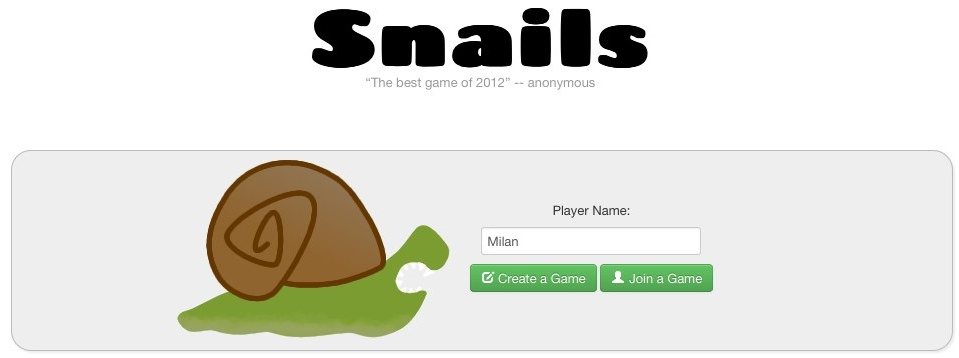
\includegraphics[width=1.0\textwidth]{index.jpg}
\caption{The welcome page}
\end{figure}

\begin{figure}[htb]
\centering
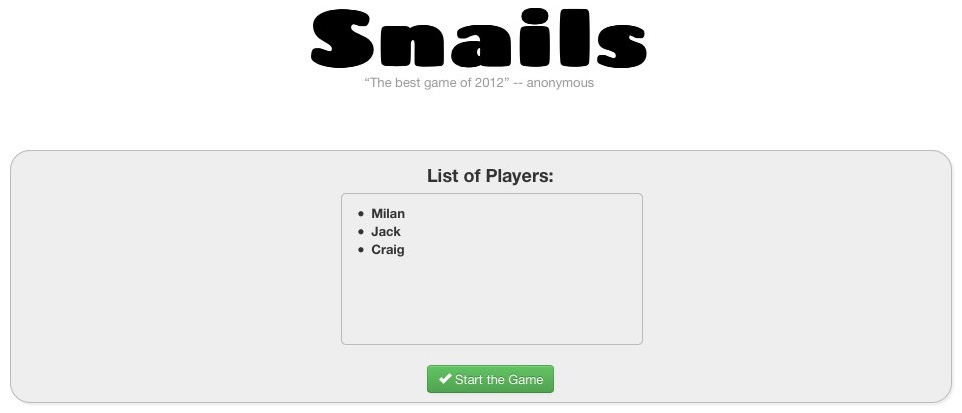
\includegraphics[width=1.0\textwidth]{create.jpg}
\caption{The screen for creating a game}
\end{figure}

\begin{figure}[htb]
\centering
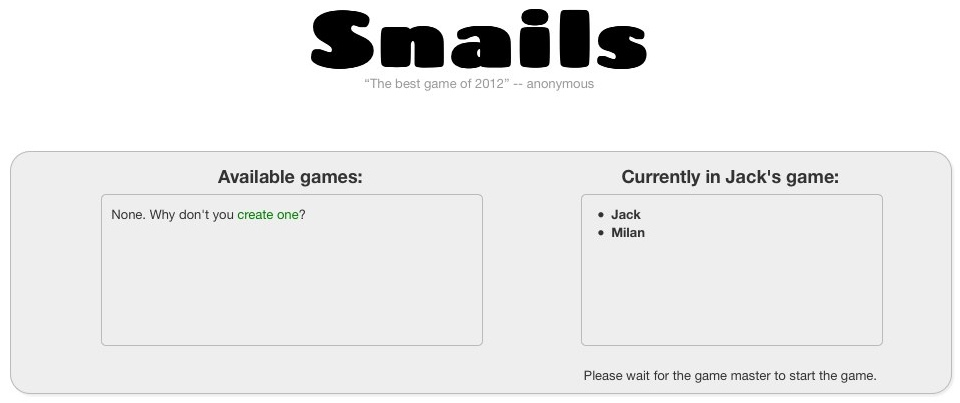
\includegraphics[width=1.0\textwidth]{join.jpg}
\caption{The screen for joining a game}
\end{figure}

\begin{figure}[htb]
\centering
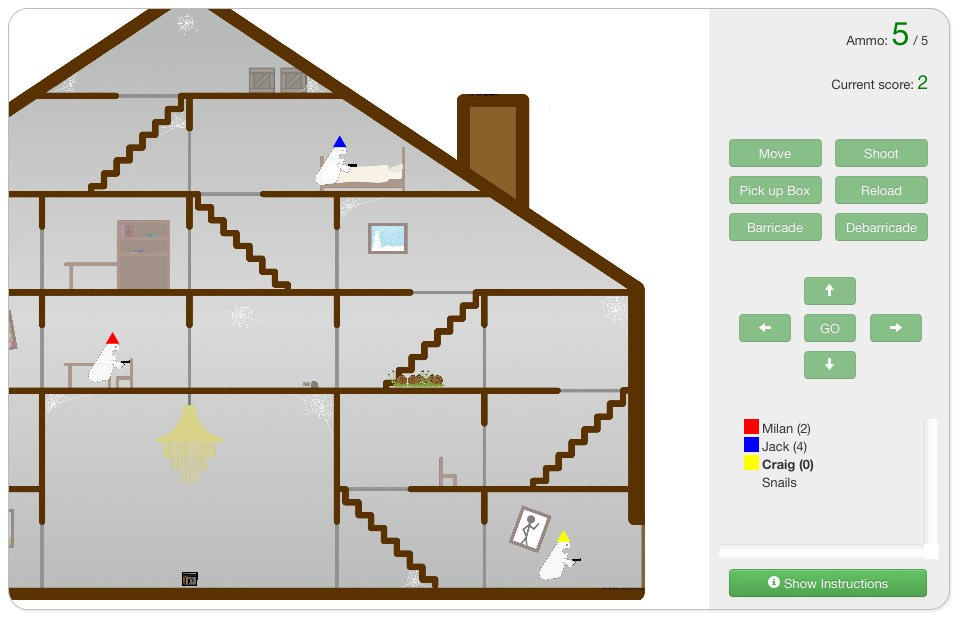
\includegraphics[width=1.0\textwidth]{game-1.jpg}
\caption{Game}
\end{figure}

\begin{figure}[htb]
\centering
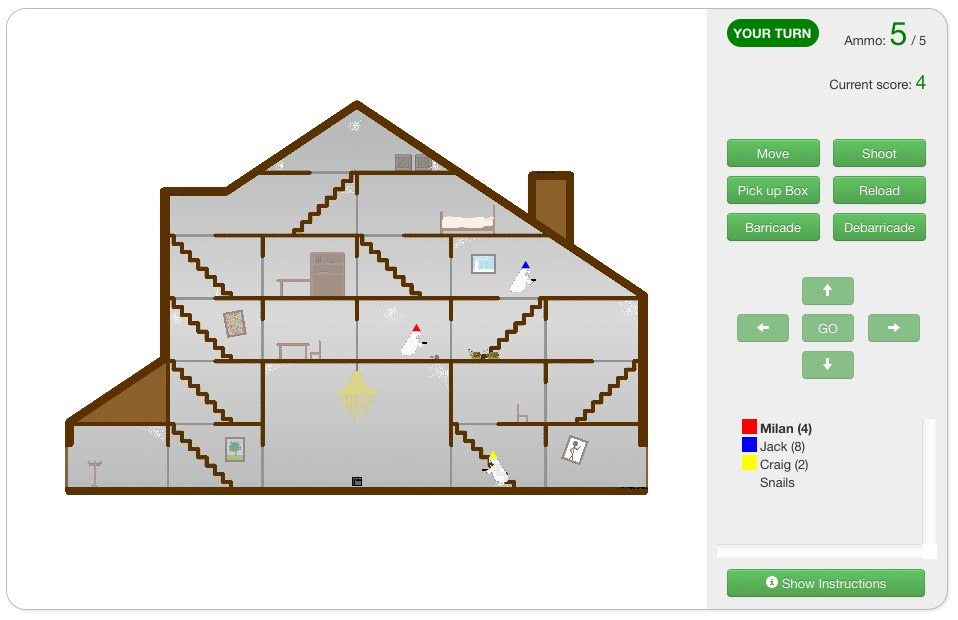
\includegraphics[width=1.0\textwidth]{game-2.jpg}
\caption{Game}
\end{figure}

\begin{figure}[htb]
\centering
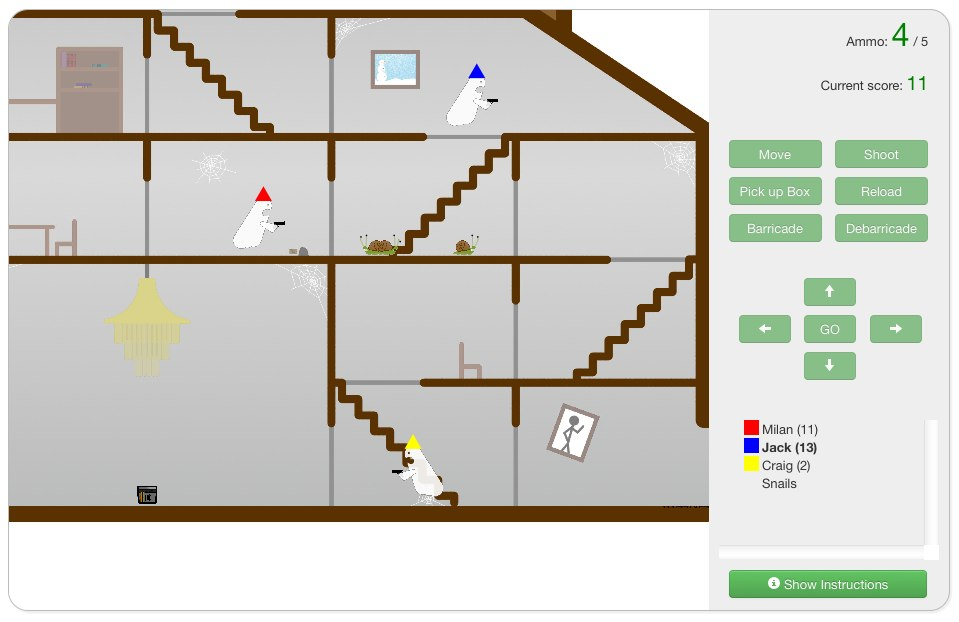
\includegraphics[width=1.0\textwidth]{game-3.jpg}
\caption{Game}
\end{figure}

\end{document}
